\problemname{Adolescent Architecture 2}

\newcommand{\playerA}{Peter}
\newcommand{\playerB}{Amy}

Three years ago, you helped little \playerA{} stack his toy blocks into a tower.
Since then, he has extended his collection of toy blocks, which now features the following base shapes:
\begin{itemize}
  \item \texttt{circle}\;$a$ -- a circle of radius $a$;
  \item \texttt{square}\;$a$ -- a square with side length $a$;
  \item \texttt{triangle}\;$a$ -- an equilateral triangle with side length $a$.
\end{itemize}
Here, $a$ may be any positive integer.
The top shapes of each block are the same as their bottom shapes,
so the blocks are cuboids, cylinders, and triangular prisms, respectively.
\playerA{} has an infinite supply of blocks of each shape and size.

\begin{figure}[h]
	\centering
	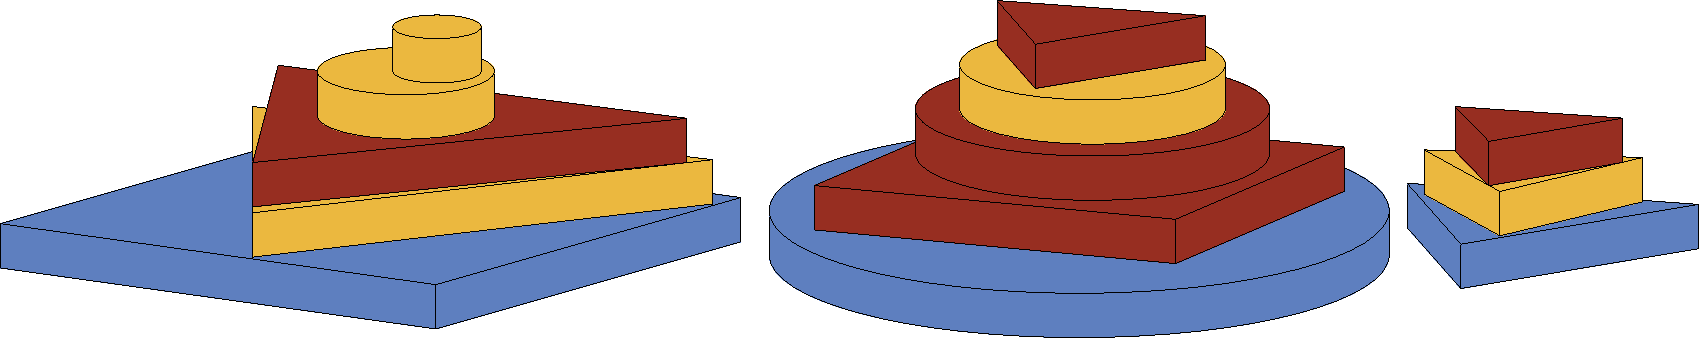
\includegraphics[width=0.8\textwidth]{image}
	\caption{A game in progress.}
\end{figure}

\playerA{} and his friend \playerB{} are playing a two-player game, where the blocks need to be stacked on top of each other.
Initially, some blocks are already placed on the floor.
In each move, the current player must take a toy block from the infinite supply and put it on top of one of the existing stacks of blocks.
The block may be rotated around its vertical axis before placing it.
The outline of the new block must be strictly within the outline of the old block; the outlines are not allowed to touch.
The first player who is unable to make a move loses the game.

Given the initial configuration, determine the number of winning moves for the first player.

\vspace{-3mm}
\begin{Input}
  The input consists of:
  \begin{itemize}
    \item One line with an integer $n$ ($1 \le n \le 1000$), the number of initial stacks.
    \item $n$ lines, each with a string~$s$ ($s$ is one of ``\texttt{circle}'', ``\texttt{square}'' or ``\texttt{triangle}'') and an integer~$a$ ($1 \le a \le 10^9$), giving the topmost blocks of the initial stacks~as~described~above.
  \end{itemize}
\end{Input}

\vspace{-3mm}
\begin{Output}
  Output the number of winning moves for the first player.
\end{Output}

\begin{afterSample}
  \section*{Notes}
  \begin{figure}[h]
    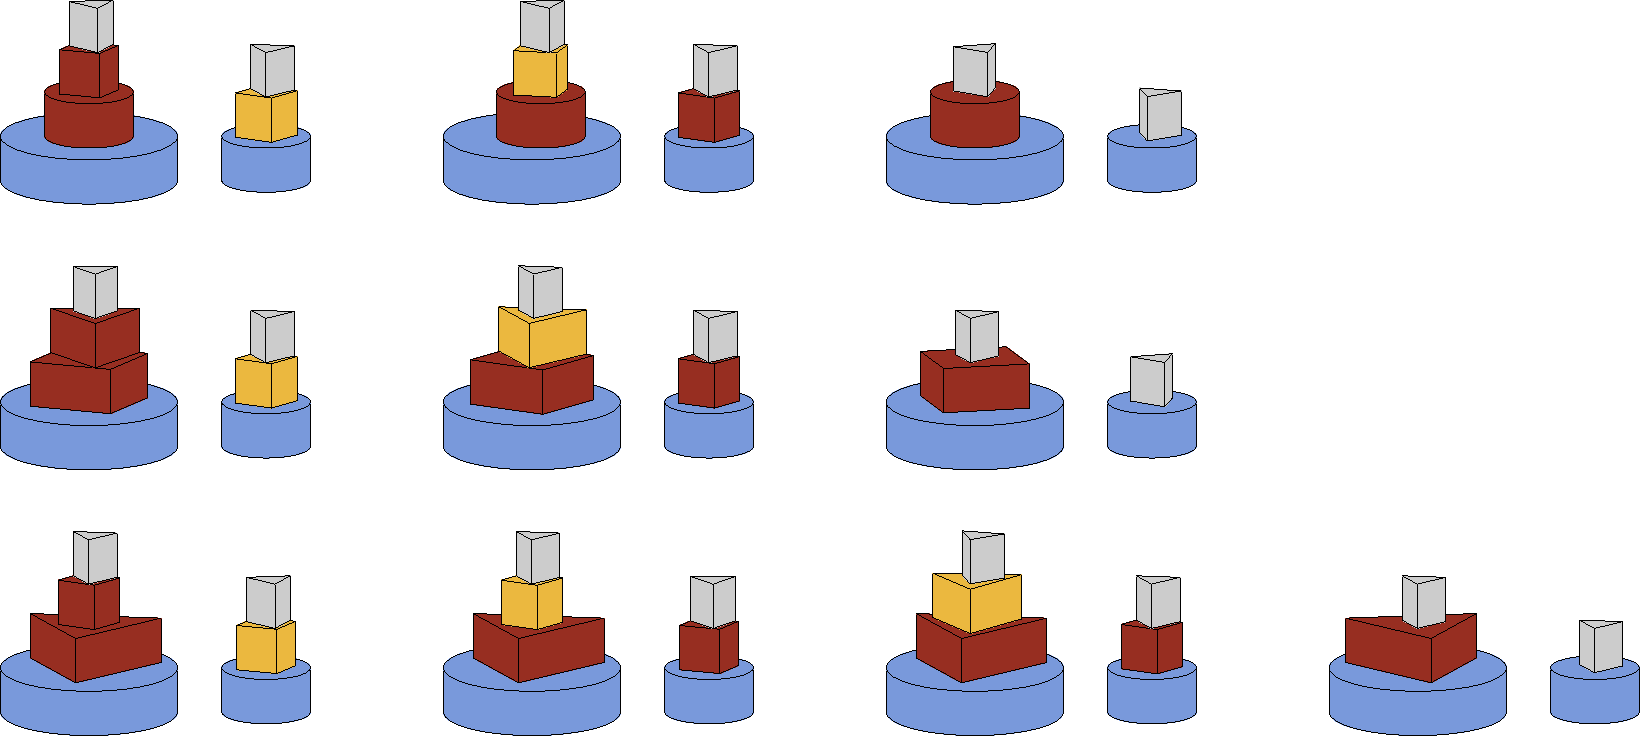
\includegraphics[width=\textwidth]{sample2}
    \vspace{3mm}
    \caption{
      Illustration of Sample Input 2, showing all possible end configurations of the game when \playerA{}
      went first and played optimally to win. The blue blocks are the initial configuration.
      \playerA{} needs to put one of \texttt{circle 1}, \texttt{square 2} or \texttt{triangle 3}
      on top of \texttt{circle 2} in order to win.
      Each of these options corresponds to one row of the figure.
      Blocks placed by \playerA{} are coloured in red, and blocks placed by \playerB{} are coloured in yellow.
      As the last two blocks are always of type \texttt{triangle 1}, they are shown in grey.
      If, for instance, \playerA{} first puts \texttt{circle 1} (as depicted in the first row),
      then \playerA{} can win by mirroring the following moves by \playerB{}.
    }
  \end{figure}
\end{afterSample}
